\subsection{Models}
In this section, we define a number of models to which we will be referring throughout the dissertation. Those models are either meant to generate synthetic data for simulations or are crafted to expose a specific aspect of an algorithm.

\subsubsection{Simple Switching Model}
The \textit{Simple Switching Model} consists of two states whose Bernoulli distributions are defined by
\begin{align*}
	\prob{X_t = 0}{C_t = 1} &= 1 \quad
	 \text{i.e.} \quad X_t \, | \, C_t = 1 \, \sim \text{Ber}(0) \\
	\prob{X_t = 1}{C_t = 2} &= 1 \quad
	\text{i.e.} \quad X_t \, | \, C_t = 2 \, \sim \text{Ber}(1)
\end{align*}

Figure \ref{ssm_transitions} shows illustrates the transition matrix $\Gamma$; the initial distribution is defined to be $\delta = (0.1, 0.9)$
\begin{figure}
	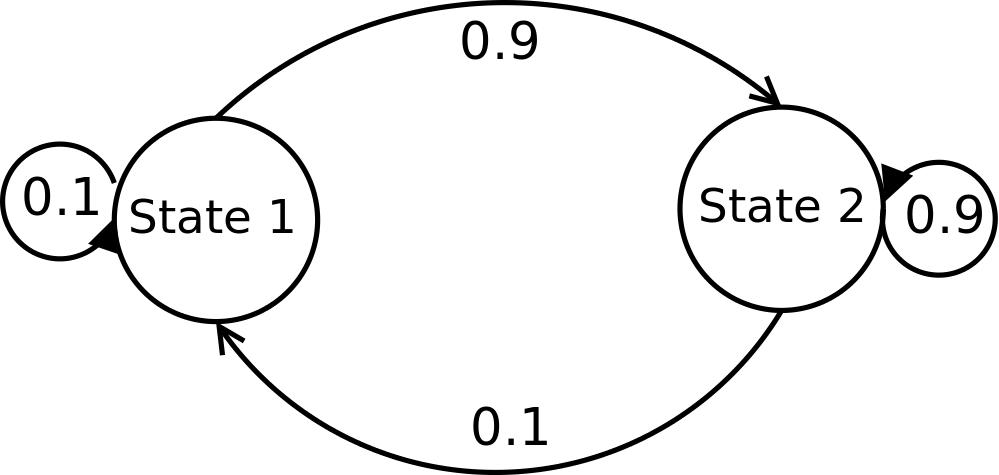
\includegraphics[width=\linewidth]{../forward_algorithm/lib/models/simpleSwitchingModel/ssm_transitions.png}
	\caption{The probabilities are crafted s.t. the system is very likely to rest permanently in state 2 and return there quickly whenever it transitions into state 1}
	\label{ssm_transitions}
\end{figure}